%% paper preamble
\documentclass[10pt,a4paper, twocolumn]{article}

\usepackage[utf8]{inputenc}
\usepackage[german]{babel}
\usepackage[T1]{fontenc}
\usepackage{fullpage}
\usepackage{graphicx}
\usepackage{listings}
\usepackage{tcolorbox}
\usepackage{url}
\usepackage{float}
\usepackage{nameref}
%\usepackage{subcaption}
\usepackage{hyperref}
\usepackage{xcolor}

\hypersetup{
  colorlinks   = true, 	%Colours links instead of ugly boxes
  urlcolor     = red, 	%Colour for external hyperlinks
  linkcolor    = blue, 	%Colour of internal links
  citecolor   = blue 	%Colour of citations
}
\definecolor{grey}{rgb}{0.9,0.9,0.9}

\setlength{\parindent}{0pt}
\setlength{\columnsep}{0.5cm}


\usepackage{amsmath}
\usepackage[]{algorithm2e}
\usepackage[]{csquotes}
\usepackage{subfigure}

\author{Sven Fiergolla \\ 1252732 \\ s4svfier@uni-trier.de}
\title{Index Construction}

\hypersetup{
    colorlinks=true,
    linkcolor=black,
    urlcolor=blue
}

\begin{document}

\LinesNumbered
\maketitle

\section{Einführung}
\paragraph{}
Information Retrieval, zu deutsch Informationsrückgewinnung, ist ein Fachgebiet, welcher sich mit computergestütztem Suchen nach komplexen Inhalten befasst. Der häufigste Anwendungsbereich ist das Suchen von Dokumenten aus einer Sammlung, die für einen Anwender relevant sind. Würde dies auf der unveränderten Datenmenge geschehen, müsste bei jeder Suchanfrage, die komplette Menge an Rohdaten durchsucht werden. Dies ist ein sehr ressourcenintensiver Prozess, daher wird zunächst auf die Hardware selbst eingegangen. Anschließend werden einige Verfahren zum Erstellen eines Index vorgestellt und auf deren Vor- und Nachteile eingegangen.\par

\section{Hardware Constraints}
\begin{figure*}[ht]
  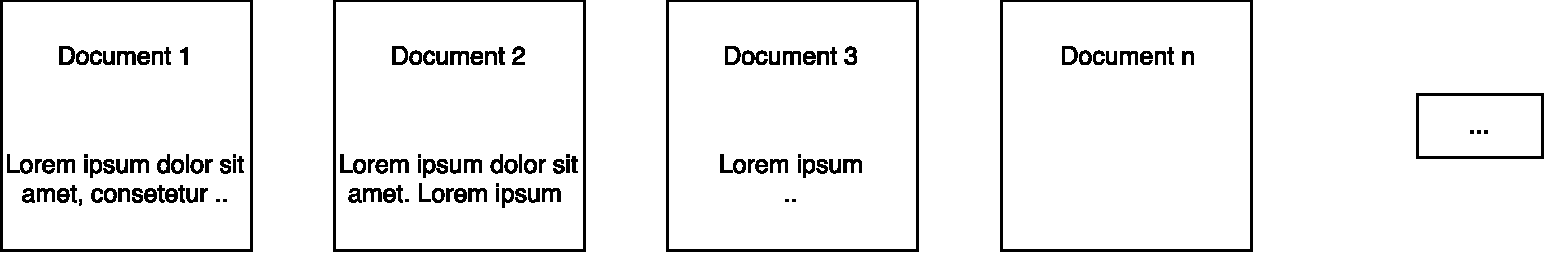
\includegraphics[width=\textwidth]{pdf/Documents.pdf}
  \caption{beispielhafter Dokumenten-Korpus}
  \label{korpus}
\end{figure*}

\paragraph{}
Typische Systemeigenschaften eines Desktop PC im Consumerbereich (Stand 2018):
\begin{itemize}
	\item \textit{clock rate} 2-4 GHz, 4-8 Kerne
	\item \textit{main memory} 4-32 Gb
	\item \textit{disk space} $\leq$ 1 TB SSD oder $\geq$ 1 TB HDD
	\begin{itemize}
	\item HDD (hard disk drive)
	\begin{itemize}
	\item \textit{average seek time} zwischen 2 und 10 ms
	\item \textit{transfer} 150 - 300 MB/s
	\end{itemize}
	\item SSD (solid state disk)
	\begin{itemize}
	\item \textit{average seek time} zwischen 0.08 und 0.16 ms
	\item \textit{transfer} Lesen: 545 MB/s, Schreiben: 525 MB/s
	\end{itemize}
	\end{itemize}
\end{itemize}	 
\par

\paragraph{}
Die zu durchsuchende Datensammlung, häufig auch Korpus genannt, befindet sich auf der Festplatte, welche deutlich langsamer arbeitet als der Arbeitsspeicher oder die CPU. Daher stellt die Festplatte in diesem Fall ein Bottleneck\footnote{Wörtlich: \enquote{Flaschenhals} oder \enquote{Engpass}. Gemeint ist ein Engpass beim Transport von Daten, der maßgeblichen Einfluss auf die Arbeitsgeschwindigkeit hat.} dar.
Um die intensive Nutzung der Festplatte zu vermeiden, wird eine alternative Datenstruktur benötigt. Je nach Anforderung kann eine andere Struktur verwendet werden. Für klassisches \enquote{Document Retrival} wird jedoch in der Regel ein so genannter Invertiert Index konstruiert (siehe \nameref{invertedIndex}).
Da sich mit der SSD eine neue Speichertechnologie verbreitet hat, welche deutlich bessere Zugriffszeiten hat als eine HDD, wird diese separat betrachtet (siehe \nameref{indexSSD}).
\par

\section{Index Construction} \label{IndexConstruction}
\paragraph{}
Um das ressourcenintensive Durchsuchen der Rohdaten zu vermeiden, existieren geeignete Datenstrukturen um Anfragen beantworten zu können, ohne alle Daten durchsuchen zu müssen. Eine einfache geeignete Struktur wäre eine \enquote{Term-Dokument-Matrix}, welche spaltenweise die Dokumente auflistet und zeilenweise das Vorkommen einzelner Wörter. Auf einer solchen Matrix lässt sich mit einfachen boolschen Anfragen arbeiten, jedoch hat diese Datenstruktur auch einige Nachteile. Beipsielsweise wächst die Matrix zu stark an für große Sammlungen, es lassen sich keine Komplexeren Anfragen stelle und ein Ranking der Dokumente ist ebenfalls nicht möglich. Daher betrachten wir im Folgenden lediglich den invertierten Index als geeignete Datenstruktur.
\par

\paragraph{}
Um aus einer Sammlung von Rohdaten (Abbildung \ref{korpus}) die relevanten Informationen zu gewinnen, müssen vorher einige Anpassungen getätigt werden. Besteht die Sammlung beispielsweise aus Webseiten, müssen die Informationen vor dem Indizieren aus der \textit{.html}-Datei geparst und von html-Tags befreit werden. In der Regel wird ebenfalls Tokenization und Stemming auf den Text angewendet. Bei der Tokenisierung wird Dokument in kleinste Einheiten (meistens einzene Wörter) geteilt. Stemming erlaubt, dass verschiedene morphologische Varianten eines Wortes auf ihren gemeinsamen Wortstamm zurückgeführt werden (beispielsweise die Deklination von Wortes oder Wörter zu Wort und Konjugation von gesehen oder sah zu seh). Dies ermöglicht, dass bei einer Suchanfrage auch Dokumente gefunden werden können, in denen eine leichte Variation des gesuchten Wortes vorkommt, da beide auf den gleichen Term reduziert werden.
\par

\subsection{Invertierter Index} \label{invertedIndex}
\paragraph{}
Die wesentlichen Schritte zur Erstellung eines invertierten Index sind in Abbildung \ref{postingssList} dargestellt. Zuerst werden alle \enquote{Term-Dokument ID} Paare gesammelt. Diese werden anschließend, dem Term nach, lexikographisch sortiert. Zuletzt werden die Dokument ID's für jeden Term in einer so genannten Postingslist zusammengefasst und Statistiken wie die Frequenz eines Terms berechnet. Die Postingslisten aller Terme bezeichnet man als invertierten Index, da die Zuordnung von Dokumenten auf deren Text invertiert wurde zu der Zuordnung zwischen einem Term und dessen Vorkommen. Sie enthalten zusätzlich statistische Information wie die Anzahl der Dokumente in welchen sie vorkommen. Bei einer Suchanfrage muss nun lediglich die Postingsliste zu dem gesuchten Term zurückgegeben werden. Aus Performancegründen werden häufig eindeutige Term ID's statt den Termen selbst genutzt. Für kleine Sammlungen kann dies im Arbeitsspeicher geschehen, für größere Sammlungen werden jedoch alternative Verfahren benötigt, auf die im Folgenden eingegangen wird.
\par

\begin{figure*}[ht]
  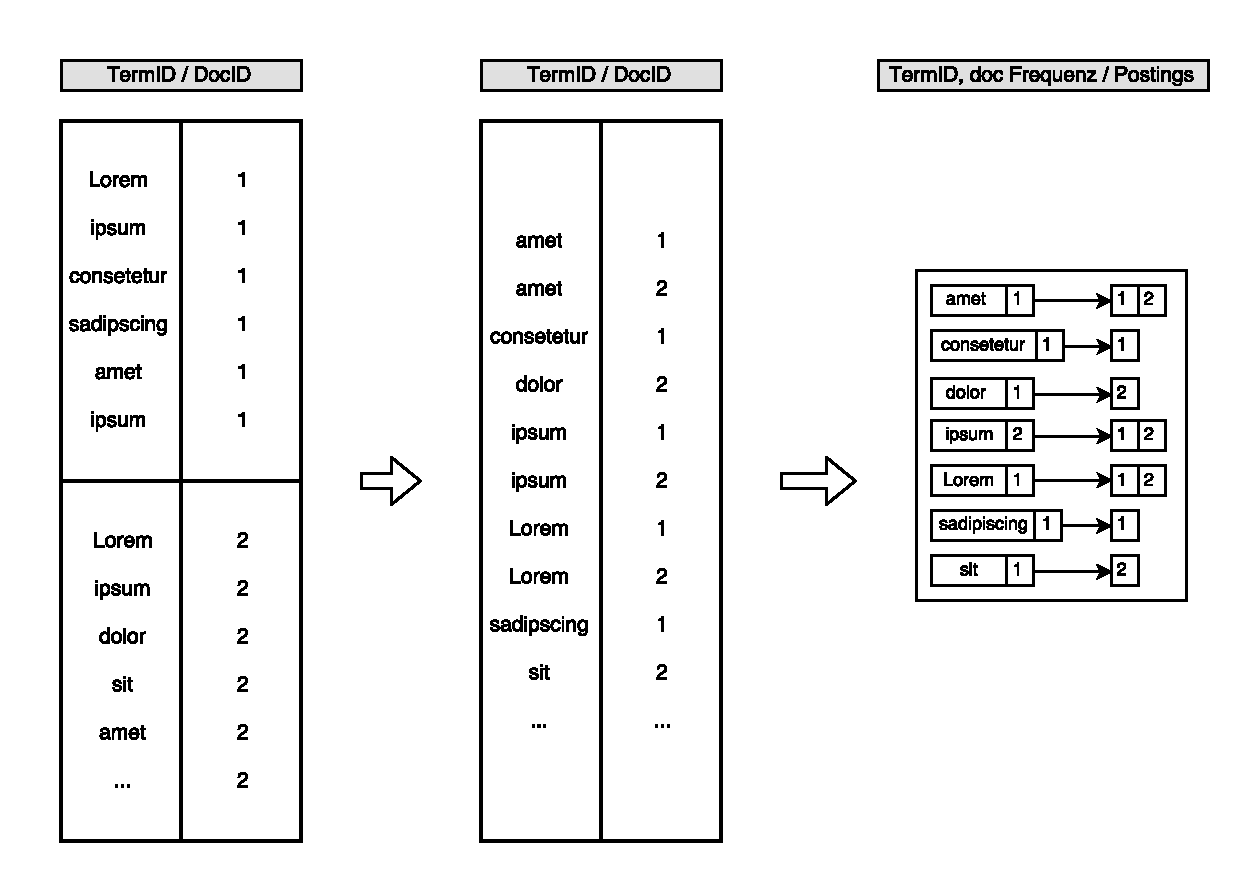
\includegraphics[width=\textwidth,height=0.45\textheight]{pdf/postingslist3.pdf}
  \caption{Invertierter Index}
  \label{postingssList}
\end{figure*}

\paragraph{}
In \enquote{Introduction to Information Retrieval}\cite{ir} wird mit einer Modellsammlung gearbeitet, der Reuters-RCV1. Sie umfasst rund $800.000$ Nachrichtenartikel aus einem Zeitraum von einem Jahr, ist etwa 1 GB groß und besitzt $100.000.000$ Terme. Die \enquote{Term-Dokument ID} Paare dieser Sammlung auf einer Festplatte zu sortieren ist sehr ineffizient. Beim Sortieren kann von einer theoretischen Komplexität von $O(n \cdot log_2 (n))$ ausgegangen werden. Möchte man nun alle Terme der Reuters-RCV1 Sammlung sortieren und man von 2 Zugriffen auf die Festplatte beim Sortieren sowie einer durchschnittlichen Zugriffszeit auf die Festplatte von 5 ms ausgeht, dauert es in etwa:

\[(100.000.000 \cdot log_2 (100.000.000)) \cdot 2 \cdot (5 \cdot 10^{-3}) \]
\[ = 2.6575424759... \cdot 10^7 \text{ Sekunden}\]
\[ = 307.59 \text{ Tage} \]

Diese Dauer resultiert vor allem aus der hohen Zugriffszeit einer mechanischen Festplatte, da bei jedem wahlfreiem Zugriff der Lesekopf neu positioniert werden muss. Das Lesen von sequenziellen Daten ist deutlich schneller. Ein erster Ansatz dieses Problem zu umgehen ist es, den wahlfreien Zugriff zu minimieren und die Daten vorzugsweise Blockweise zu lesen.
\par

\subsection{Blocked sort-based indexing}
\paragraph{}
Eine Ansatz dies zu umgehen ist den Index Blockweise zu erstellen mit Hilfe des \textit{block sort-based indexing Algorithmus} (siehe Algorithmus \ref{bsbiAlgo}) oder auch \textit{BSBI} auf welchen im Folgenden näher eingegangen wird.
\par
\begin{algorithm}
 n = 0\;
 \While{all documents have not been processed}{
n = n + 1\;
block = ParseNextBlock()\;
BSBI-INVERT(block)\;
WriteBlockToDisk(block, $f_n$)\;
  }
  MergeBlocks($f_1$, $\cdots$, $f_n$; $f_{merged}$)\;
\caption{BSBI Algorithmus} \label{bsbiAlgo}
\end{algorithm}

\paragraph{}
Der Algorithmus parst eine Menge von Dokumenten in \enquote{Term-Dokument ID} Paare bis ein Block mit einer festen Größe voll ist (Zeile 4). Anschließend wird der Block sortiert, daher sollte der Block problemlos in den Arbeitsspeicher passen, da dieser wesentlich schneller arbeitet als die Festplatte und so ein effizienteres Sortieren ermöglicht wird. Nun wird ein invertierter Index für den Block erstellt und persistiert (Zeile 5). Dies geschieht iterativ für alle Blöcke bis die Sammlung komplett bearbeitet wurde. Zuletzt werden die einzelnen Postingslist zusammengefügt (Zeile 8) bis alle Listen in einen Invertierten Index über alle Dokumente gemerged wurden (siehe Abbildung \ref{bsiMerging}). 
\par

\begin{figure*}[ht]
  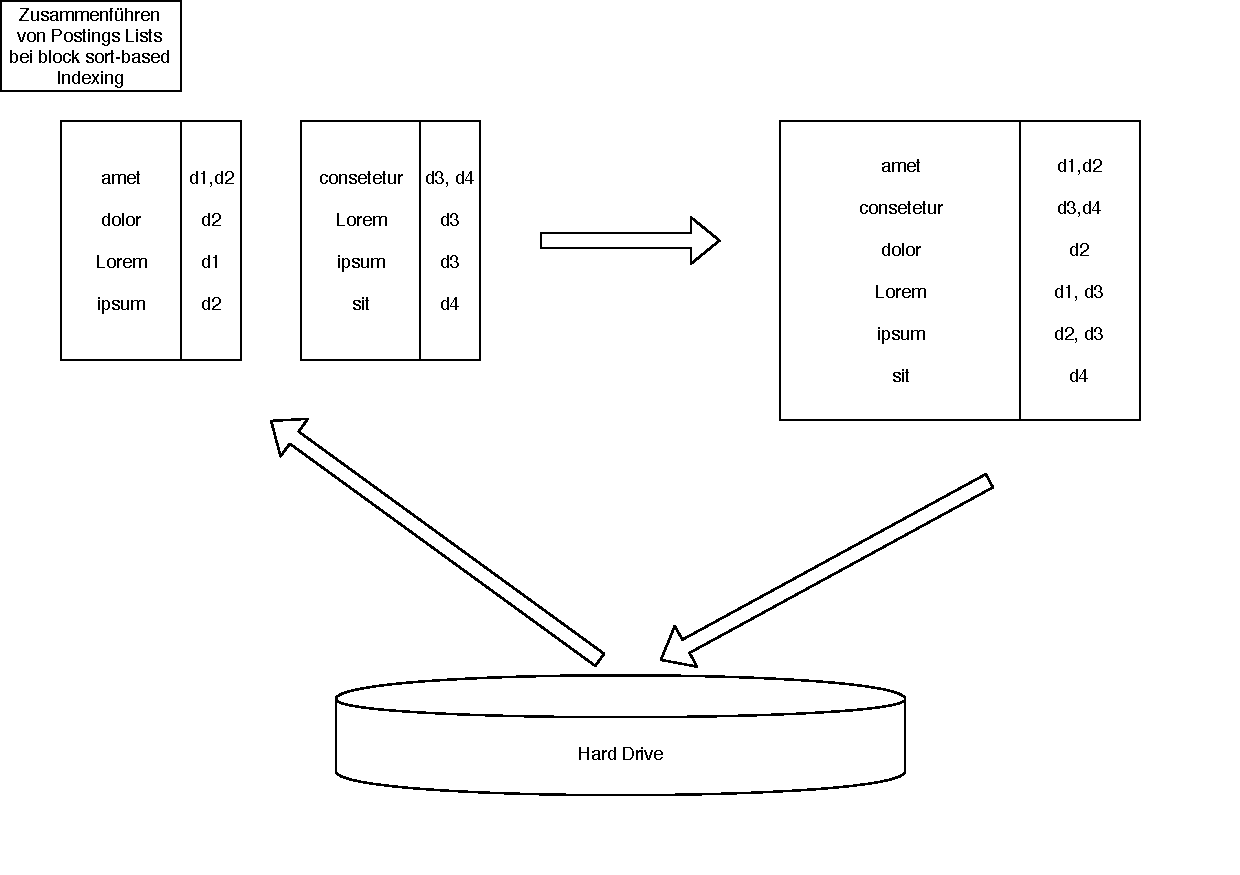
\includegraphics[width=\textwidth]{pdf/BSI_merging.pdf}
  \caption{merging bei BSBI}
  \label{bsiMerging}
\end{figure*}

\paragraph{}
Soll über die Reuters-RCV1 Sammlung mit BSBI ein Index erstellt werden, so dauert dies unter gleichen Voraussetzungen nur noch 15,5 Stunden, da die Sammlung in 64 Blöcke aufgeteilt wird. Diese können innerhalb des Arbeitsspeichers sortiert werden, welcher eine wesentlich bessere Zugriffsgeschwindigkeit vorweist. Dennoch ist die theoretische Zeitkomplexität von BSBI $\Theta( T\cdot log_2( T))$ da die $T$ Terme sortiert werden müssen, auch wenn dies innerhalb eines Blocks geschieht. In der Praxis ist jedoch meistens das Parsen und Mergen der Blöcke am zeitaufwendigsten. Zudem wird mit Term-ID's gearbeitet, daher muss zusätzlich eine Datenstruktur für das Mapping zwischen Termen und Term-ID's im Arbeitsspeicher gehalten werden.\par

\subsection{Single-pass in-memory indexing}
\paragraph{}
BSBI lässt sich für viele Sammlungen anwenden, benötigt jedoch eine Datenstruktur für die Zuordnung zwischen Termen und ihren Term-ID's. Eine alternative Umsetzung ist der \textit{single-pass in-memory indexing Algorithmus} oder auch \textit{SPIMI} (siehe Algorithmus \ref{spimiAlgo}). Anders als bei BSBI werden bei SPIMI Terme statt Term-ID's betrachtet, daher kann auf ein Mapping wie bei BSBI verzichtet werden. Zudem werden die Terme in einem Dictionary gehalten und beim Auftreten der Postingslist angehangen, sodass auf das Sortieren der Terme verzichtet werden kann. Das Dictionary ist eine einfach geordnete Datenstruktur für das Mapping zwischen einem Term und dessen Hash, welche für jeden Block separat erstellt wird.\par

\paragraph{}
 Die Sammlung von Dokumenten wird als Datenstrom\footnote{Als Datenstrom (Englisch: data streams) bezeichnet man einen kontinuierlichen Fluss von Datensätzen, dessen Ende meist nicht im Voraus abzusehen ist.} von \enquote{Term-Dokument ID} Paaren betrachtet und darauf wiederholt der Algorithmus angewendet, bis die ganze Sammlung indiziert wurde. Wenn ein Term innerhalb eines Bocks zum ersten mal vorkommt, wird er dem Dictionary hinzugefügt (Zeile 6 und Abbildung \ref{fig:subfigure1}) und eine neue Postingsliste wird erstellt. Kommt ein Term wiederholt vor, so wird über das Hash des Dictionary auf die Postingsliste zugegriffen (Zeile 8 und Abbildung \ref{fig:subfigure2}) und das neue Vorkommen als Posting der Liste hinzugefügt. Da die Länge der Postingsliste nicht dynamisch ist, muss sie bei Bedarf verdoppelt werden (Zeile 11). Wenn der verfügbare Arbeitsseicher verbraucht ist, wird das Dictionary und die Postingslisten des Blocks persistiert und ein neuer Block geparst und bearbeitet (Zeile 17). Die Terme müssen sortiert im Dictionary vorliegen, da die Postingslisten dann in lexikoraphischer Ordnung persistiert werden können. Wurden alle Blöcke bearbeitet, werden die einzelnen Postingslisten zusammengeführt. Dies ist deutlich effizienter wenn sich die Postingslisten der einzelnen Blöcke bereits in lexikographischer Ordnung befinden.\par

\paragraph{}
Anders als BSBI kann SPIMI über beliebig große Sammlungen einen Index erstellen, solange das Festplattenvolumen nicht überschritten wird, da keine weitere Datenstruktur für die Zuordnung zwischen Termen und ihren Term-ID's im Arbeitsspeicher gehalten werden muss. Zudem können die bearbeiteten Blöcke größer sein, da weniger Arbeitsspeicher verbraucht wird, was die Indexerstellung als ganzes effizienter macht. Ein weiterer Aspekt ist Komprimierung, das Dictionary eines Blocks und die Postingslisten können so besonders kompakt gespeichert werden. Da die Terme sortiert in das Dictionary eingefügt werden und somit das Sortieren der Terme ausbleibt sind alle Operationen von SPIMI linear, die Zeitkomplexität beträgt $\Theta(T)$ mit $T$ als Anzahl der Terme der Sammlung.

\subsection{Distributed indexing}
\paragraph{}
BSBI und SPIMI eignen sich gut für Datensammlungen, die von einem Rechner verarbeitet werden können. Übersteigt der Umfang der Sammlung jedoch die Rechenleistung eines einzelnen Rechners, muss ein Index über solch eine Sammlung auf andere Weise erstellt werden. Das Web umfasst ca.\ eine Millarden Webseiten und muss daher von einem Computer-Cluster bearbeitet werden. Ein Computercluster oder Rechnerverbund bezeichnet eine Menge von vernetzten Computern. Solche Cluster bieten die Möglichkeit eine \textit{MapReduce}-Architektur anzuwenden, eine generelle Architektur für verteiltes Arbeiten. So können aufwendige Probleme von vielen, günstigen Rechnern, auch \textit{Nodes} genannt, gelöst werden. Ein einzelner Rechner wird zum \textit{Master-Node}, welcher für das Verteilen der einzelnen Aufgaben verantwortlich ist. Da einzelne Nodes jederzeit ausfallen können, muss der Master-Node Aufgaben jederzeit neu zuweisen können.\par

\paragraph{}
Wird ein Index auf einem solchen verteiltem System erstellt, ist auch der Index selbst geteilt (siehe \nameref{distribIndex}). Dies geschieht entweder nach Dokumenten oder nach Termen. Wird der Index nach Dokumenten geteilt, bearbeiten unterschiedliche Maschinen des Clusters unterschiedliche Abschnitte der Sammlung und erstellen einen Index für jeden Abschnitt welche abschließend zusammengeführt werden. Häufig wird der Index jedoch auch nach Termen geteilt, diese Herangehensweise wird im Folgenden näher beschrieben. Da der Index verteilt erstellt wird, ist auch die Zuordnung zwischen Termen und ihren Term-ID's verteilt und daher komplexer. Eine einfache Lösung ist es, die Zuordnung für häufige Terme im Voraus zu berechnen und auf alle Nodes zu verteilen. Für seltene Terme können die Terme statt Term-ID's verwendet werden.\par

\paragraph{}
Zu Beginn wird die Sammlung in $n$ gleiche Teile unterteilt, die sogenannten \textit{Splits}. Ein Ansatz ist es, die Anzahl der Splits gleich der Anzahl an Nodes zu wählen, so kann jedem Node genau ein Split zugeordnet werden. Alternativ sollte die Größe eines Splits so gewählt werden, dass die Arbeit gleich verteilt werden kann und ein Split von einem herkömmlichen Rechner in einer kurzen Zeit bearbeitet werden kann (16 oder 64MB pro Split). Während der ersten Phase von MapReduce, der \textit{Map-Phase} wird jedem Node ein Split zugewiesen und geparst. Die Ausgabe der $r$ Nodes wird in $j$ lokale Hilfsdateien gespeichert, welche auch \textit{segment files} genannt werden. Sie beinhalten die Postings je eines lexikographischen Abschnitts von Termen eines Splits, was es ermöglicht diese später sequenziell auszulesen. In der \textit{Reduce-Phase} weist der Master-Node je einen der $j$ lexikographischen Abschnitte einem Node zu, welcher alle $r$ segment files dieses Abschnittes zusammenführt. Abschließend werden die verbundenen und sortierten Postingslisten persistiert (siehe \enquote{postings} in Abbildung \ref{distribIndex}).\par

\subsection{Dynamic indexing} \label{Section:dynamicIndex}
\begin{figure*}[ht]
  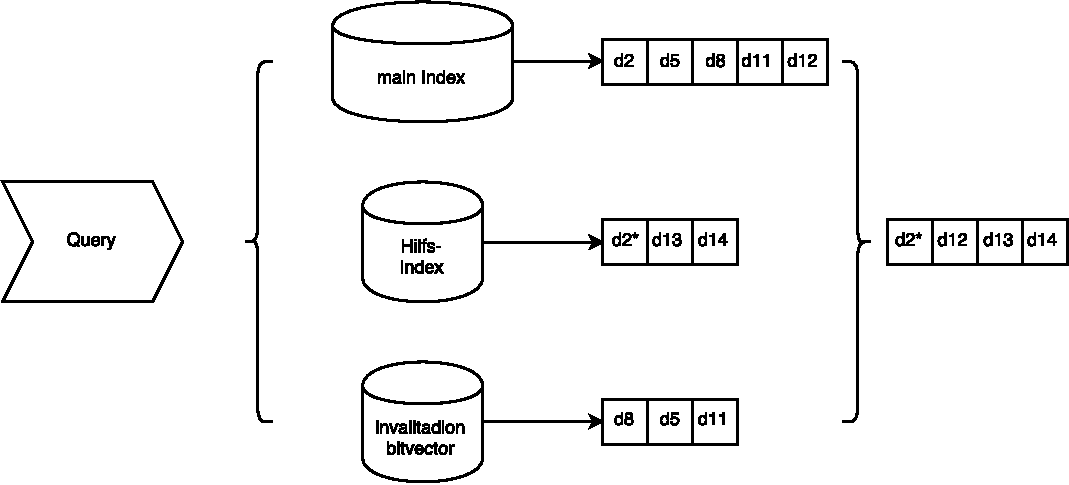
\includegraphics[width=\textwidth,height=.25\textheight]{pdf/dynIndexCrop.pdf}
  \caption{Query auf einem dynamic index}
  \label{dynIndex}
\end{figure*}

\paragraph{}
In den bisher vorgestellten Indexierungsverfahren wurde von einer statischen Sammlung mit statischen Inhalten ausgegangen. Viele Sammlungen sind jedoch sehr dynamisch und ändern sich häufig, Webseiten beispielsweise werden geändert, gelöscht oder es werden neue hinzugefügt. Sollten die Änderungen nicht sehr gravierend sein, kann es reichen periodisch einen neuen Index zu erstellen und damit den alten Index zu ersetzten. Müssen die Änderungen jedoch sofort sichtbar sein, muss der Index über eine solche dynamische Sammlung ebenfalls dynamisch sein.\par

\paragraph{}
Dazu erstellt man sich einen Hauptindex der die wesentlichen Informationen enthält und einen Hilfsindex, welcher Änderungen enthält. In einem einfachen Bit-Vektor werden gelöschte Dokumente eingetragen. Wird der Hilfsindex zu umfangreich, werden Haupt- und Hilfsindex zusammengeführt, dabei werden auch als gelöscht markierte Dokumente aus dem Index entfernt. Der Aufwand dieser merge-Operation hängt stark von der Art der Speicherung der Indexes ab. Ist jede Postingslist eine eigene Datei so muss lediglich die Postingsliste des Hauptindex um die zugehörige Postingsliste aus dem Hilfsindex erweitert werden. In diesem Fall ist der Nutzen des Hilfsindex lediglich den Zugriff auf die Festplatte zu minimieren, da so nur beim Zusammenführen der Indizes zusätzlicher Festplattenzugriff stattfindet. Viele Betriebssysteme können jedoch nicht effizient mit einer sehr großen Menge an Dateien umgehen. In der Praxis wird daher häufig eine Konkatenation der einzelnen Postingslisten aller Dokumente, aufgeteilt auf wenige Dateien, verwendet.\par

\paragraph{}
Anfragen werden gegen beide Indizes und den Bit-Vektor ausgeführt. Trifft ein Dokument auf eine Query zu, so wird dieses zurückgegeben. Falls Änderungen in dem Dokument sind, wird das geänderte Dokument aus dem Hilfsindex und nicht aus dem Hauptindex zurückgegeben. Sollte das Dokument als gelöscht markiert im Bit-Vektor vorliegen, so wird es aus der Ergebnismenge  gefiltert. Das Ausführen einer Query auf einem dynamischen Index ist ebenfalls in Abbildung \ref{dynIndex} visualisiert.\par

\paragraph{}
In dieser Herangehensweise muss beim Mergen jeder der  $T$ Terme $ \lfloor \frac{T}{n}\rfloor$ mal betrachtet werden, bei eine Größe $n$ des Hilfsindex. Daher beträgt die theoretische Zeitkomplexität dieses Zusammenführens $\Theta(\frac{T^2}{n})$. Diese Zeitkomplexität kann durch das Einführen von weiteren Hilfsindizes $I_0 , I_1 , I_2  \dots $ der Größe $2^0 \times n, 2^1 \times n, 2^2 \times n\dots$ und sogenanntes \textit{logarithmic merging} verbessert werden. Wie zuvor werden bis zu $n$ Postings in einem Hilfsindex $Z_0$ gespeichert. Ist dieser voll, werden die $2^0 \times n$ Postings in einen Index $I_0$ auf der Festplatte transferiert. Ist $Z_0$ erneut voll, so wird dieser mit Index $I_0$ zu Index $Z_1$ der Größe $2^1 \times n$. Existiert noch kein Index $I_1$, so wird $Z_0$ zu $I_1$, andernfalls wird $Z_0$ mit $I_1$ zusammengeführt und zu $Z_2$. Dieses Verfahren gilt für alle Iterationen des Index. Um eine Query auszuwerten, muss diese gegen $Z_0$ und alle validen Indizes $I_i$ ausgeführt werden, die Ergebnisse werden zusammengeführt. Die Zeitkomplexität dieser Herangehensweise beträgt $\Theta (T \cdot log(\frac{T}{n}))$, da jedes Posting nur ein mal auf jeder der $log(\frac{T}{n})$ Ebenen betrachtet werden muss. Diese gewonnene Effizienz bei der Erstellung des Index resultiert jedoch aus einer langsameren Ausführung einer Query auf diesem Index, da nun mehrere Indizes durchsucht werden müssen.\par

\subsection{andere Indexierungsverfahren}
\paragraph{}
Neben den bisher vorgestellten Verfahren zum Erstellen eines Index, welche unterschiedliche funktionale Aspekte aufwiesen, existieren noch weitere, auf welche hier nur kurz eingegangen wird.\par

\paragraph{}
Häufig wird statt \textit{boolean retrieval} ein \textit{ranked retrieval} umgesetzt, sodass bei einer Anfrage eine Ordnung nach Relevanz gegeben werden kann. In diesem Fall werden die Postings nach einer Gewichtung sortiert in die Postingsliste aufgenommen. Werden bei einer Anfrage lange Postingslisten für einen Term gefunden, müssen diese nicht vollständig durchsucht werden, da die weiteren Postings der Dokumente von niedriger Relevanz nicht benötigt werden. Dies erschwert jedoch das Erweitern eines solchen Invertierten Index, da die Postings für neue Dokumente an beliebiger Position in die Postingsliste eines Terms aufgenommen werden können.\par

\paragraph{}
Sicherheit spielt vor allem in betrieblich oder kommerziell genutzten Indizes eine Rolle, in denen verschiedene Nutzergruppen unterschiedliche Rechte zum Auslesen des Index besitzen. Dazu werden die Zugriffsrechte der Nutzergruppen in einer \textit{acces controll list}, einer einfachen Matrix mit dem Schema Nutzer $\times$ Dokumente gespeichert. Die Ergebnismenge wird nach dem Ausführen einer Query nach dieser Matrix gefiltert, sodass der Nutzer nur Dokumente finden kann, auf welche er auch Zugriffsrecht hat.\par

\paragraph{}
In \enquote{Managing Gigabytes: Compressing and Indexing Documents and Images}\cite{managingGig} wird eine Herangehensweise zur \enquote{in situ}-Erstellung eines Index vorgestellt. Dabei wird mit einer minimalen Anzahl an Hilfsdateien gearbeitet, sodass bei der Erstellung nicht mehr Speicherplatz verbraucht wird als der finale Index groß ist. Dies findet vor allem in der wachsenden Zahl an \enquote{embedded systems} Anwendung, da diese über sehr limitierte Hardware verfügen.\par

\section{Indexierung mit Solid State Drives} \label{indexSSD}

\begin{figure*}[ht]
  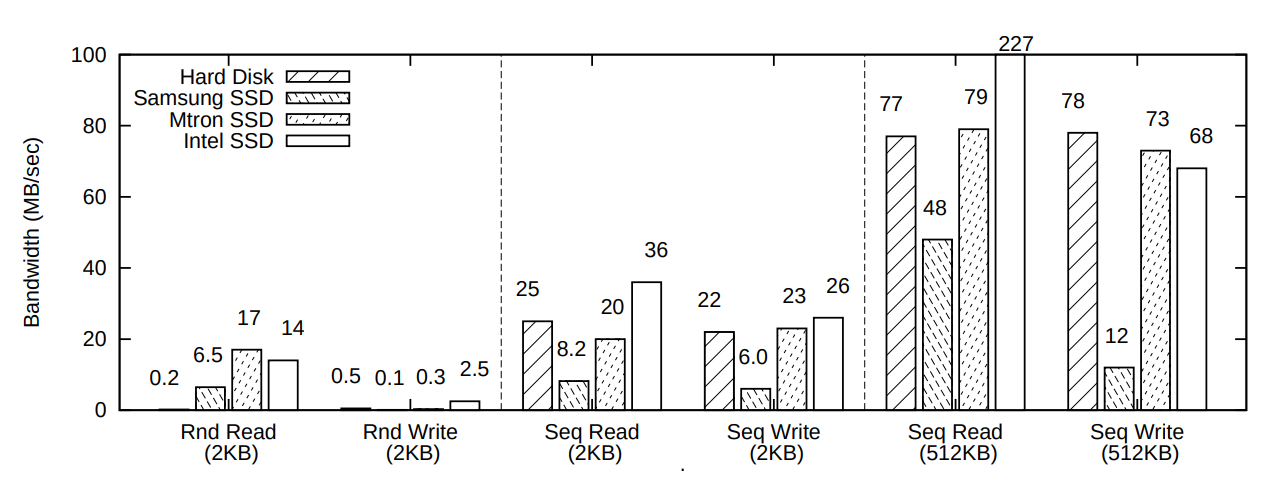
\includegraphics[width=\textwidth,height=.29\textheight]{pdf/ssdperformance.png}
  \caption{Zugriffsgeschwindigkeit verschiedener SSD's bei unterschiedlichen Aufgaben sowie einer HDD als Referenz}
  \label{fig:accessSSD}
\end{figure*}

\paragraph{}
Seit geraumer Zeit setzten sich \textit{Solid State Drives} (SSD) gegenüber herkömmlichen mechanischen Festplatten auf dem Markt durch, da sie über immer mehr Datenvolumen verfügen, weniger Energie verbrauchen und sich preislich angleichen. Viele Algorithmen, besonders die zur Erstellung eines Index, hatten als funktionale Anforderung die Minimierung des Festplattenzugriffs, da besonders der wahlfreie Zugriff durch das Positionieren des Lesekopfs sehr langsam ist. In der Arbeit \enquote{Indexing on Solid State Drives}\cite{ssd} wurden dazu die Zugriffszeiten verschiedener Festplatten gemessen, darunter eine günstige SSD von Samsung, eine herkömmliche SSD von Mitron und eine teure SSD von Intel sowie eine HDD als Referenzwert. Wie aus der Abbildung ersichtlich ist, sind auch bei SSD's die sequenziellen, schreibenden Zugriffe (Abbildung \ref{fig:accessSSD}, mitte 2KB \& rechts 512KB) deutlich schneller sind als ein wahlfreier Zugriff (Abbildung \ref{fig:accessSSD}, links). Diese Eigeschaft resultiert aus dem sogenannten \enquote{erase before write}-Mechanismus von \textit{EEPROM} oder \enquote{electrically erasable programmable read only memory} Speichertechnologien wie der SSD. Soll ein Sektor des Flashspeichers, auch Page genannt, beschrieben werden und es befinden sich bereits Daten darauf muss, auch wenn diese als gelöscht markiert wurden, die komplette Page gelöscht und mit 1 überschrieben werden. Dies muss geschehen, da die Schreibeoperation auf Grund der technischen Realisierung dieser Speichermedien nur bits von 1 zu 0 ändern können. Diese Eigenschaft verlangsamt das Speichermedium wenn häufig wahlfreie schreibende Zugriffe erfolgen.\par

\paragraph{}
Da vorallem Baumindizes die primäre Zugriffsmethode für Datenbanken sind, gilt es diese an die neue Hardware anzupassen. Der klassische B+ Baum als Datenstruktur für mechanische Festplatten, funktioniert grundsätzlich auch auf einer SSD. Ein B+ Baum ist Erweiterung eines immer vollständig balancierten Baumes, der Daten nach Schlüsseln sortiert speichert. Durch die Sortierung ist das Suchen in einem solchen Baum sehr effizient. Suchoperationen werden durch die schnellen, wahlfreien lesenden Zugriffe begünstigt, Updateoperationen werden jedoch langsamer. Um dieses Problem zu umgehen wird in \enquote{Indexing on Solid State Drives}\cite{ssd} ein sogenannter FD-Baum als geeignete Datenstruktur vorgeschlagen (siehe Abbildung \ref{FD Tree}).\par

\paragraph{}
Um die Updateperformace des Indexes zu verbessern während die Sucheffizienz beibehalten werden soll, wird eine logarithmische Datenstruktur gewählt um den Aufwand eines Updates gering zu halten. Das \textit{logarithmic merging} von Updates ist bereits aus \nameref{Section:dynamicIndex} bekannt und wird hier ebenfalls verwendet. Die Baumstruktur selbst besteht aus einem kleinen B+ Baum als oberste Ebene (genannt \textit{head tree}), über mehreren sortierten Ebenen welche nach untern in der Größe zunehmen. Je ein Blatt des Baums besitzt die Größe einer Page der Festplatte. Über \enquote{Fences} wird auf andere Blätter anderer Ebenen mit Indexeinträgen referenziert um im Baum zu suchen. Mit Hilfe von \textit{fractional cascading} wird die Suche weiter beschleunigt. Fractional cascading bietet die Möglichkeit, die Bereichssuche in einem Bereichsbaum schneller zu gestalten. Dabei wird der jeweils höchstdimensionale assoziierte Baum nicht als Baum, sondern als Array gespeichert. Von jedem Element des Arrays gehen Verweise auf mindestens gleich große Schlüsselwerte in den beiden Kindarrays. Updates werden nur im head tree getätigt und iterativ in die unteren sortierten Ebenen eingefügt. Dies hat zur Folge, dass die meisten wahlfreien Zugriffe zu sequenziellen Zugriffen auf die Festplatte werden.\par

\paragraph{}
Auf einem FD-Baum mit $n$ Einträgen und einer Page-Größe von $B$ lässt sich analytisch zeigen, dass eine Update-Operation in $\mathcal{O}(log_B(n))$ sequenziellen Festplattenzugriffen und das Ausführen einer Query in $\mathcal{O}(log_B(n))$ wahlfreien Zugriffen erfolgt. Damit hat der FD-Baum eine vergleichbare Suchperformance wie der standart B+ Baum und eine ähnliche Update-Performance wie die für schreibenden Zugriff optimierte B+ Baum Variante. Dies zeigt, dass die Gesamtperformance des FD-Baums über den anderen B+ Baum Varianten liegt, vorallem auf SSD's jedoch auch auf mechanischen Festplatten.\par 

\paragraph{}
Zwischen den SSD's verschiedener Modelle und Hersteller bestehen jedoch gravierende Unterschiede wie die Page-Größe und die verwendeten Hardwarecontroller. Um dem entgegen zu wirken, wurde als Teil der Arbeit zusätzlich ein Kostenmodel entwickelt um die optimale Größe der sortierten Ebenen an die jeweilige Festplatte anzupassen und die Performance so noch weiter zu steigern.\par

\section{Fazit}
\paragraph{}
Grundsätzlich erfordern unterschiedliche Anforderungen unterschiedliche Indexierungsverfahren. Auf einzelnen Rechnern lassen sich mit Hilfe von BSBI oder SPIMI auf einfache Weise ein invertierter Index erstellen, SPIMI ermöglich dies sogar in linearer Zeitkomplexität. Für größere Datenmengen wie das Web oder sehr dynamische Sammlungen müssen andere Architekturen verwendet werden um den Anforderungen gerecht zu werden, doch mit MapReduce und logarithmischem zusammenführen von Hilfsindizes ist dies ebenfalls möglich. Da sich die Hardware jedoch ebenfalls im Laufe der Zeit geändert hat und mit Solid State Drives eine neue Speichertechnologie durchgesetzt hat, müssen für mechanische Festplatten entwickelte Algorithmen neu überdacht werden. Mit Hilfe eines FD-Baumes, der speziell für neue Speichermedien konzipiert wurde, ist dies im Bereich der Indexerstellung geschehen.\par

\paragraph{}
Abschließend lässt sich sagen, dass für gängige Anforderungen eine geeignetes Indexierungsverfahren und eine Indexstruktur existiert. Die Menge an Daten welche Weltweit gesammelt und gespeichert wird wächst jedoch weiter und es kommen neue, gänzlich unterschiedliche Ansätze für Information Retrieval bzw.\ Document Retrieval auf. Der Einsatz von künstlicher Intelligenz zeigt auch in diesem Bereich Erfolge. Multimedia Information Retrieval, wie das Suchen nach Bildern und Videos anhand von Ähnlichkeit oder anderen nicht textuellen Aspekten, lässt sich mit neuen Modellen und Ansätzen lösen.
\par

\begin{thebibliography}{9}

		\bibitem{ir}
		Christopher D. Manning, Prabhakar Raghavan and Hinrich Schütze \enquote{\href{https://nlp.stanford.edu/IR-book/pdf/04const.pdf}{Introduction to Information Retrieval}}  Cambridge University Press 2008, pp. 1-18 and 67-84.

	 \bibitem{managingGig}
	  Ian H. Witten, Alistair Moffat, Timothy C. Bell \enquote{\href{https://books.google.de/books?id=2F74jyPl48EC&dq=Witten+et+al.+index+1999&lr=&hl=de&source=gbs_navlinks_s}{Managing Gigabytes: Compressing and Indexing Documents and Images}}  Morgan Kaufman Publishers 1999, pp. 223-261.
	
	\bibitem{ssd}
	Yinan Li, Bingsheng He, Robin Jun Yang, Qiong Luo, Ke YiTree (Hong Kong University of Science and Technology) \enquote{\href{http://pages.cs.wisc.edu/~yinan/paper/fdtree_pvldb.pdf}{Indexing on Solid State Drives}} The 36th International Conference on Very Large Data Bases, September 13-17,
2010, Singapore.
\end{thebibliography}

%\newpage

\section*{Appendix}
\subsubsection*{Single-pass in-memory indexing Algorithmus}

\begin{algorithm}
\emph{SPIMI-Invert(token\_ stream)}\\
 outputFile = new File()\;
 dictionary = new HashFile()\;
 \While{free memory available}{
 token = next(TokenStream)\;
\eIf{term(token) $\notin$ dictionary}{
PostingsList = AddToDictionary(dictionary, term(token))\;
}{
PostingsList = GetPostingsList(dictionary, term(token))\;
}
\If{full(PostingsList)}{
PostingsList = DoublePostingsList(dictionary, term(token))\;
}
AddToPostingsList(PostingsList, docID(token))\;
  }
SortedTerms = SortTerms(dictionary)\;
WriteBlockToDisk(SortedTerms, dictionary, OutputFile)\;

  \caption{SPIMI-invert Algorithmus} \label{spimiAlgo}
\end{algorithm}

\pagebreak
\newpage


\begin{figure*}[ht]
       \subfigure{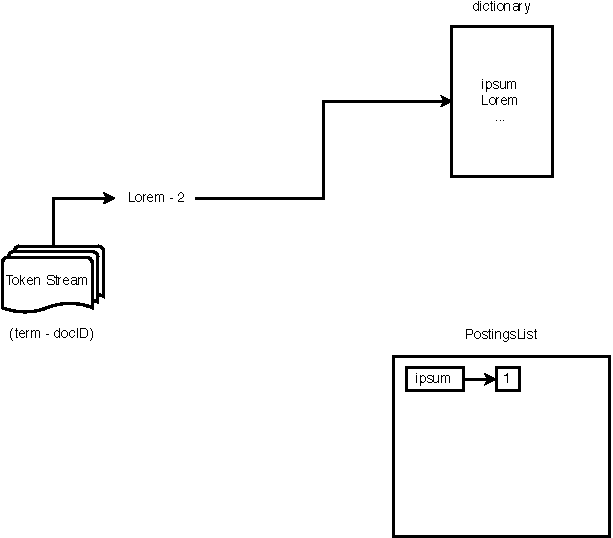
\includegraphics[height=.46\textheight]{pdf/spmi-crop1.pdf}}
        \subfigure{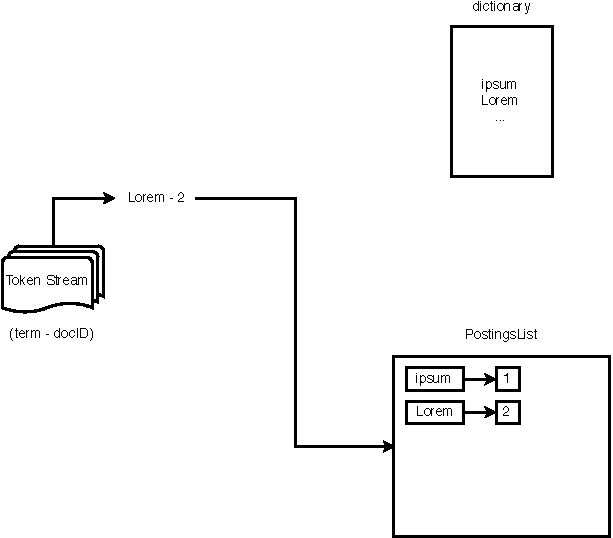
\includegraphics[height=.46\textheight]{pdf/spmi-crop2.pdf}}
    \caption{Erstes Auftreten eines Terms. Term wird Dictionary hinzugefügt und Postingsliste wird erstellt.}
   \label{fig:subfigure1}
\end{figure*}


\begin{figure*}[ht]
        \subfigure{
            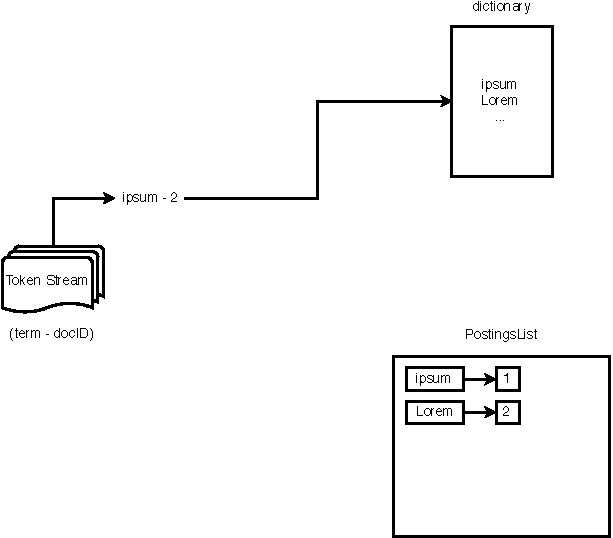
\includegraphics[height=.46\textheight]{pdf/spmi-crop3.pdf}
        }
        \subfigure{
           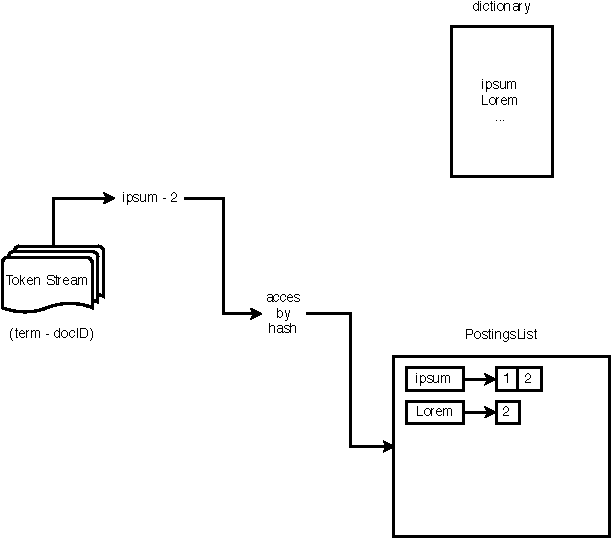
\includegraphics[height=.46\textheight]{pdf/spmi-crop4.pdf}
        }
    \caption{ Wiederholtes Auftreten eines Terms. Term wird in Dictionary gefunden und per Hash der Postingsliste des Terms hinzuefügt.}
   \label{fig:subfigure2}
\end{figure*}

\begin{figure*}[hb]
  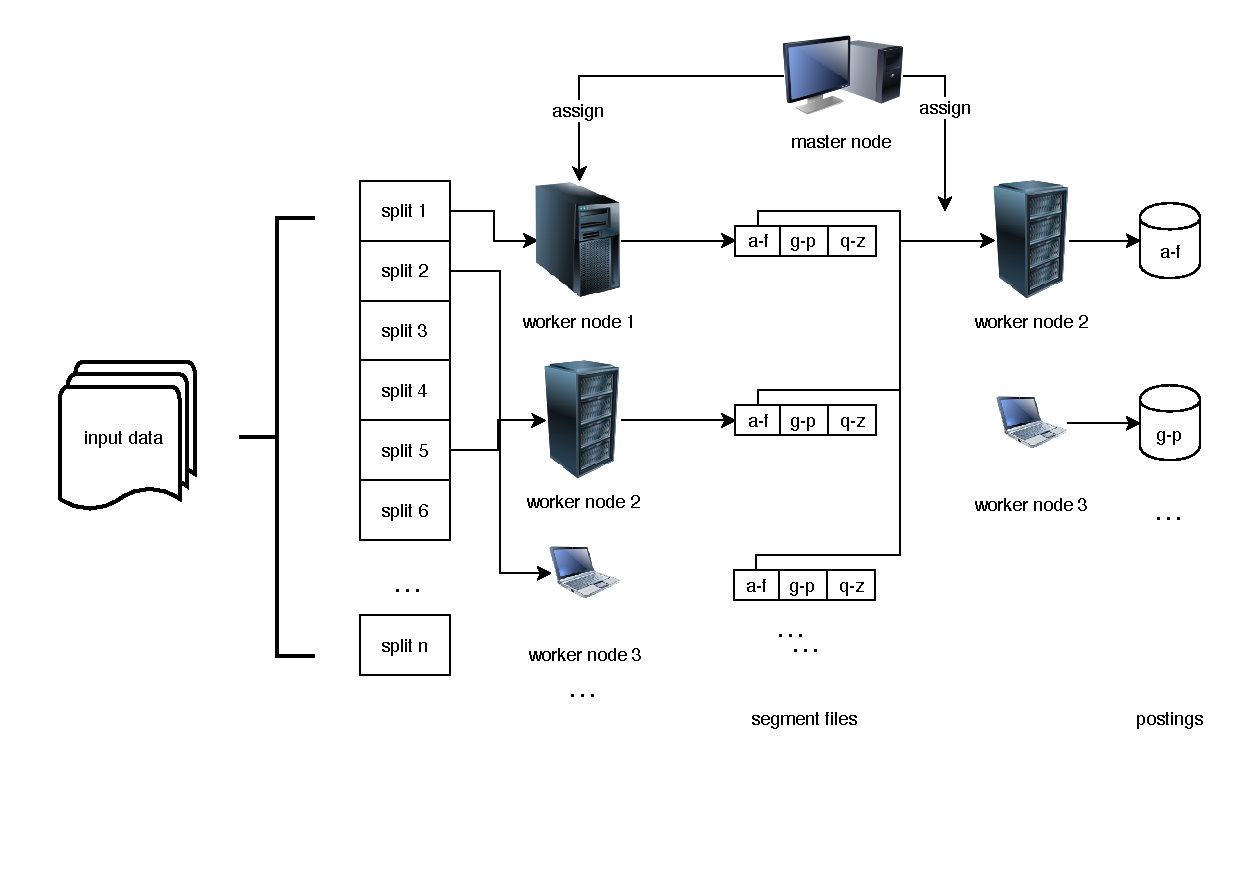
\includegraphics[width=\textwidth]{pdf/distributedIndexAll.pdf}
  \caption{distributed indexing mit MapReduce}
  \label{distribIndex}
\end{figure*}

\begin{figure*}[ht]
  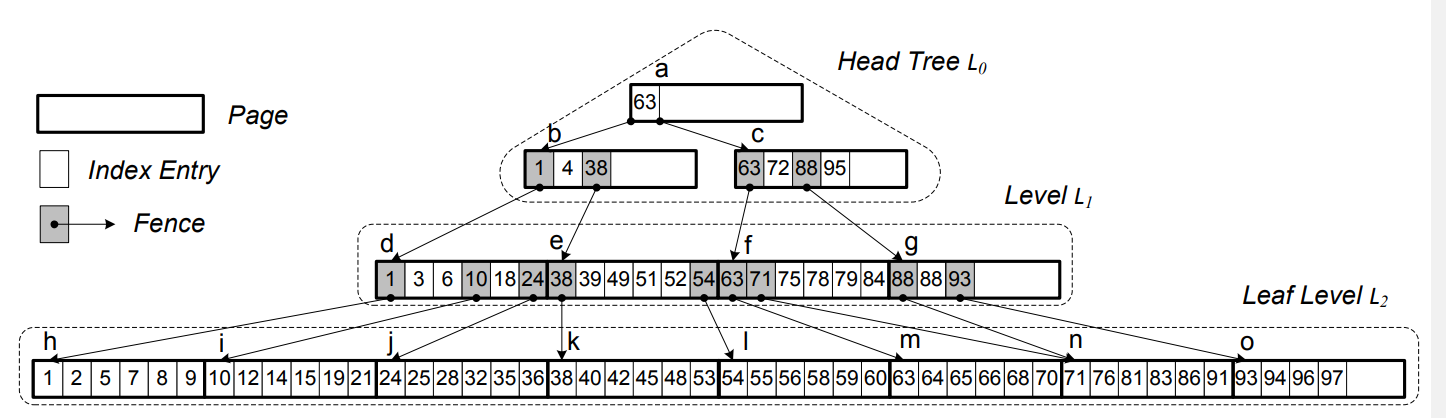
\includegraphics[width=\textwidth]{pdf/fdtree.png}
  \caption{FD-Baum, tree index}
  \label{FD Tree}
\end{figure*}

\end{document}